% Drawing 74/05-14 -- folder 74, batch 05, archive page 88 (PDF page 89).
% Transcription: Un carré de sommets $x$, $y$ (en haut), $y'$, $x'$ (en bas), avec ses deux diagonales ; une flèche $u$ va de $x$ à $y$.
% Kind: square with diagonals and an arrow u. Method 2 (schematic redraw from the facsimile). Status: ok.
% Notes: Square x, y (top), y', x' (bottom) with its two diagonals; the arrow u from x to y along the top side.
% Coordinates: 1 unit = 1 mm = 1/100 of the crop width (bbox in page fractions: [0.15, 0.52, 0.32, 0.61]).
% Redrawn by Claude (claude-opus-5-5), issue #73, 2026-11-07; not checked by a human; not compiled (no TeX in the session).
% Rights: reproduces part of the work -- behind RENDER_TRANSCRIPTS, never published by itself.
\documentclass[tikz,border=3pt]{standalone}
\usepackage{amsmath,amssymb}
\usetikzlibrary{patterns,arrows.meta}
\tikzset{pencil/.style={black!45}, struck/.style={black!35}, mark/.style={circle,draw,inner sep=1.3pt}, pt/.style={circle,fill,inner sep=0.9pt}, opt/.style={circle,draw,fill=white,inner sep=1.1pt}}
\begin{document}
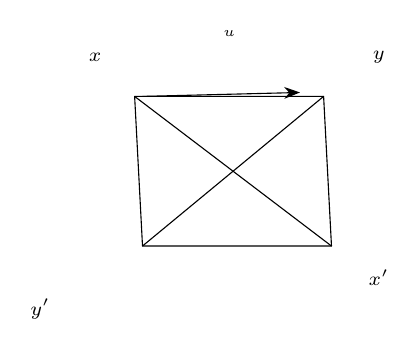
\begin{tikzpicture}[x=1mm,y=1mm,line cap=round,line join=round,font=\scriptsize]
\draw (43,-31) -- (67,-31) -- (68,-50) -- (44,-50) -- cycle;
\draw (43,-31) -- (68,-50);
\draw (67,-31) -- (44,-50);
\draw[-{Stealth[length=2mm]}] (44,-31) -- (64,-30.5);
\node[inner sep=1pt] at (38,-26) {\scriptsize $x$};
\node[inner sep=1pt] at (74,-26) {\scriptsize $y$};
\node[inner sep=1pt] at (31,-58) {\scriptsize $y'$};
\node[inner sep=1pt] at (74,-54) {\scriptsize $x'$};
\node[inner sep=1pt] at (55,-23) {\tiny $u$};
\end{tikzpicture}
\end{document}
